\documentclass[english,12pt,a4paper]{article}

\usepackage[T1]{fontenc}
\usepackage[english]{babel}
\usepackage[left=1.5cm, right=1.5cm, top=2cm, bottom=2cm]{geometry}
\usepackage{graphicx}
\usepackage{mathtools}
\usepackage{amssymb}
\usepackage{nameref}
\usepackage{hyperref}
\usepackage{titlesec}

\setcounter{tocdepth}{3}

\addto{\captionsenglish}{
	\renewcommand{\contentsname}{Summary}
}

\title{Robot : "Fancy clock"}
\author{Jory Lafaye}
\date{\today}

\begin{document}
\maketitle
\tableofcontents
\listoffigures
\listoftables
\newpage

\section{Introduction}

	The objective of this project is to model and control a Pybricks motor. The clock hand is designed to be very lightweight, so that external mechanical effects can be neglected.
	
	The system uses a Medium Powered Up™ motor, which is a DC motor equipped with an internal gearbox. Although such motors exhibit typical nonlinear behaviors, these effects significantly influence the motor dynamics and must therefore be properly modeled.
	
	Once the model is established, the motor will be controlled in torque to demonstrate a clock that completes a full cycle in 10 seconds. The clock hand will complete one full rotation before quickly returning backward to its initial position.
	
	In the following sections, we will first derive the state-space model of the motor. Then, experiments will be conducted to identify the physical parameters. Finally, a control strategy will be implemented to achieve the desired clock motion.
	
	\begin{figure}[h]
		\centering
		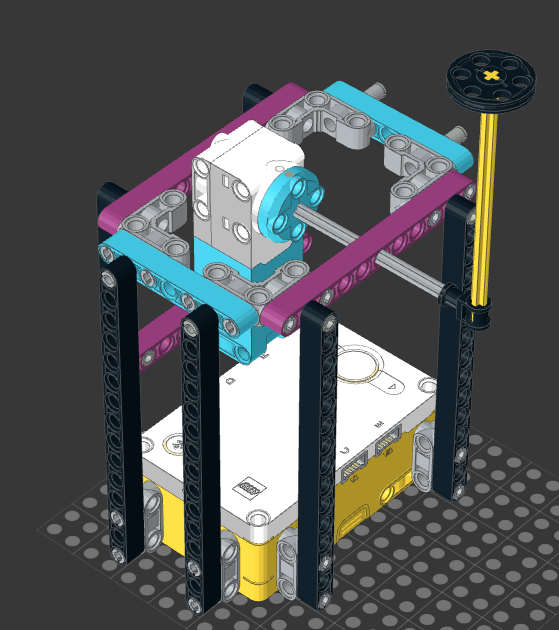
\includegraphics{robot_3d_view.png}
		\caption{3D view of the robot}
	\end{figure}
	
\section{Continuous-Time modeling}

	The Pybricks firmware provides an internal sensing system that publishes the end shaft angle, angular velocity, and estimated load torque at a frequency of 100 Hz.
	
	Communication between the embedded system and ROS is achieved via Bluetooth Low Energy (BLE) using the GATT protocol. This communication introduces a significant and variable delay, with an average latency of approximately 30 ms. The delay is measured in real time.
	
	The motor is controlled by specifying a maximum voltage along with a duty cycle percentage, which determines the applied PWM signal.
		
	Several significant nonlinear behaviors must be considered:
	\begin{itemize}
		\item \textbf{Viscous friction (gearbox):} The gearbox introduces viscous friction, which can be modeled as a torque opposing the motion and proportional to the angular velocity of the output shaft.
		
		\item \textbf{Dry (Coulomb) friction:} The gearbox also generates dry friction. When the motor torque is below a certain threshold, no motion occurs. This effect can be modeled as a constant opposing torque with a bounded magnitude.
		
		\item \textbf{Mechanical backlash:} The gearbox exhibits backlash, which can be modeled using a virtual angle directly driven by the motor and assumed to be free of mechanical friction (negligible compared to gearbox friction). The motion of the output shaft then depends on the relative position of this virtual angle.
		
		\item \textbf{Electrical viscous friction:} The motor also exhibits an electrical damping effect, which can be modeled as a viscous friction opposing the motion of the virtual angle and proportional to its angular velocity.
	\end{itemize}
	
	Depending on the experimental results, the model may be refined to better capture these non-linearities or to include additional dynamics, such as electrical inductance effects.	
	
	\subsection{State variables}

		To account for the non-linearities, the following state variables are defined:
		\begin{itemize}
			\item The angular position, velocity and acceleration of the output shaft: $q(t)$, $\dot{q}(t)$, $\ddot{q}(t)$.
			\item The angular position, velocity and acceleration of the virtual shaft: $r(t)$, $\dot{r}(t)$, $\ddot{r}(t)$.
		\end{itemize}
		
		The virtual shaft angle can be expressed as a function of the motor rotor position $r_m(t)$ and the gearbox ratio $G_m$:
		\begin{equation}
			r(t) = G_m r_m(t)
		\end{equation}
	
	\subsection{Command variables}
	
		The control input to the motor is the applied PWM duty cycle, expressed as a percentage of the maximum voltage: $p(t)$.
		
	\subsection{Observation variables}
		The Pybricks firmware provides measurements at a frequency of 100 Hz. The available observations are:
		
		\begin{itemize}
			\item The angular position and velocity of the output shaft: $q_m(t)$ and $\dot{q}_m(t)$.
			\item The estimated load torque: $\tau_m(t)$.
		\end{itemize}
		
	
	\subsection{State equations}
	
		The state dynamics can be expressed as follows:
		\begin{align}
			J_q \ddot{q}(t) &= \Gamma_{rq}(t) - \Gamma_d(t) - K_q \dot{q}(t) \\
			J_r \ddot{r}(t) &= K_m V_m p(t) - \Gamma_{rq}(t) - K_r \dot{r}(t)
		\end{align}
		where:
		\begin{itemize}
			\item $J_r$ is the rotor inertia (before the gearbox).
			\item $J_q$ is the equivalent inertia of the gearbox and external shaft.
			\item $V_m$ is the maximum voltage corresponding to 100\% duty-cycle.
			\item $K_m$ is the motor torque constant, relating the applied voltage to the generated torque (assuming negligible inductance effects).
			\item $K_r$ is the electrical damping coefficient, relating rotor velocity to an opposing torque (back-EMF effect).
			\item $K_q$ is the mechanical viscous friction coefficient associated with the gearbox and external shaft.
			\item $\Gamma_{rq}(t)$ is the torque transmitted through the gearbox, capturing nonlinear effects such as backlash and friction.
			\item $\Gamma_d$ is the dry friction induced by the gearbox.
		\end{itemize}
		
		The dry friction is modeled using a saturation function:
		\begin{equation}
			\Gamma_d(t) = \min\big(\max\big(\Gamma_{rq}(t), -\Gamma_{dM}\big), \Gamma_{dM}\big)
		\end{equation}
		where $\Gamma_{dM}$ denotes the maximum static friction torque that must be overcome to initiate motion.
		
		The coupling torque $\Gamma_{rq}$ between the rotor and the end shaft depends on the mechanical backlash and can be modeled using a piecewise model. Let $\Delta_b$ denote the half-width of the backlash dead zone, expressed at the output shaft.
		\begin{itemize}
			\item \textbf{Dead-zone (no contact):} when the relative displacement remains within the backlash gap:
			\begin{equation}
				\big|r(t)-q(t)\big| < \Delta_b,
			\end{equation}	
			there is no mechanical contact between the shafts. Consequently,
			\begin{align}
				\Gamma_{rq}(t) &= 0 \\
				\Gamma_d(t) &= 0
			\end{align}
			and the two subsystems evolve independently:
			\begin{align}
				J_q \ddot{q}(t) &= - K_q \dot{q}(t) \\
				J_r \ddot{r}(t) &= K_m V_m p(t) - K_r \dot{r}(t)
			\end{align}
			
			\item \textbf{Contact condition:} when $\big|r(t)-q(t)\big| = \Delta_b$, the shafts come into contact. The impact is assumed perfectly inelastic and damping during impact is neglected, so that the velocities instantaneously match:
			\begin{equation}
				\dot{q}(t) = \dot{r}(t).
			\end{equation}
						
			Since contact occurs on only one side of the backlash, the sign of $\Gamma_{rq}(t)$ depends on the relative position of the shafts.
			
			To determine whether contact is maintained or lost, we introduce the \emph{free accelerations} $\breve{\ddot{q}}(t)$ and $\breve{\ddot{r}}(t)$ (i.e., accelerations in the absence of coupling):
			
			\begin{align}
				\breve{\ddot{r}}(t) &= \frac{K_m V_m}{J_r} p(t) - \frac{K_r}{J_r} \dot{r}(t) \\
				\breve{\ddot{q}}(t) &= - \frac{K_q}{J_q} \dot{q}(t)
			\end{align}
			
			Assuming $\dot{r}(t) = \dot{q}(t)$ when in contact, the contact is maintained if:
			\begin{equation}
				r(t) > q(t) \text{ and}\ \breve{\ddot{r}}(t) \ge \breve{\ddot{q}}(t)
			\end{equation}
			or:
			\begin{equation}
				r(t) < q(t) \text{ and}\ \breve{\ddot{r}}(t) \le \breve{\ddot{q}}(t)
			\end{equation}
			
			Otherwise, the contact is lost and the system re-enters the backlash dead zone.
			
			These conditions can be rewritten in terms of the control input $p(t)$:
			\begin{align}
				r(t)>q(t) \text{ and}\ p(t) \ge \frac{J_r}{K_m V_m} \left( \frac{K_r}{J_r} - \frac{K_q}{J_q}  \right) \dot{q}(t) \\
				r(t)<q(t) \text{ and}\ p(t) \le \frac{J_r}{K_m V_m} \left( \frac{K_r}{J_r} - \frac{K_q}{J_q}  \right) \dot{q}(t)
			\end{align}
			
			These expressions show that if the viscous friction on the rotor dominates that of the output shaft, losing contact requires a control input of opposite sign (i.e., no control input will maintain contact).
			
			In the opposite case, a control input greater than the dry friction torque must be maintained to prevent losing contact.
			
		\end{itemize}
		
	\subsection{Model summary}
	
		The motor modeling is expressed as five different dynamics, depending on the gearbox mechanical backlash and the dry friction.
		
		
		\subsubsection{No contact in the gearbox}
			In this state, the end shaft moves freely and the rotor is directly controlled by the input duty cycle until a contact is made. The dynamic equation is expressed as follows:
			\begin{align}
				J_q \ddot{q}(t) &= - K_q \dot{q}(t) \\
				J_r \ddot{r}(t) &= K_m V_m p(t) - K_r \dot{r}(t)
			\end{align}	
			
			A contact happens when $\big|q(t)-r(t)\big| = \Delta_b$, that imply generally a discontinuity in the rotor velocity $\dot{r}(t)$, due to the inelastic impact.
			
			
		\subsubsection{Contact in the gearbox - $r(t)>q(t)$ - Control input greater than dry friction}
			In this state, the end shaft and the rotor are coupled, rigidly linking their velocity and position. The control input has to reach a minimum threshold to maintain the contact.
			\begin{align}
				q(t) &= r(t) - \Delta_b \\
				\dot{q}(t) &= \dot{r}(t) \\
				\ddot{q}(t) &= \ddot{r}(t) \\
				p(t) &\ge \frac{J_r}{K_m V_m} \left( \frac{K_r}{J_r} - \frac{K_q}{J_q} \right) \dot{q}(t) \\
				K_mV_mp(t) &\ge \Gamma_{dM} \\
				\big( J_r + J_q \big) \ddot{q}(t) &= K_mV_mp(t) - \Gamma_{dM} - \big(K_r+K_q\big)\dot{q}(t)
			\end{align}
	
	
		\subsubsection{Contact in the gearbox - $r(t)>q(t)$ - Control input lower than dry friction}
			In this state, the contact can be maintained if there is enough control input to overcome the rotor dry friction, but it does not translate to motion on the end shaft.
			\begin{align}
				q(t) &= r(t) - \Delta_b \\
				\dot{q}(t) &= \dot{r}(t) \\
				\ddot{q}(t) &= \ddot{r}(t) \\
				p(t) &\ge \frac{K_r}{K_m V_m} \dot{q}(t) \\
				K_mV_mp(t) &< \Gamma_{dM} \\
				\big( J_r + J_q \big) \ddot{q}(t) &= - \big(K_r+K_q\big)\dot{q}(t)
			\end{align}
			
			This state may not exist if:
			\begin{equation}
				K_r \dot{q}(t) > \Gamma_{dM}
			\end{equation}
			
		\subsubsection{Contact in the gearbox - $r(t)<q(t)$ - Control input greater than dry friction}
			In this state, the end shaft and the rotor are coupled, rigidly linking their velocity and position. The control input has to reach a minimum threshold to maintain the contact.
			\begin{align}
				q(t) &= r(t) + \Delta_b \\
				\dot{q}(t) &= \dot{r}(t) \\
				\ddot{q}(t) &= \ddot{r}(t) \\
				p(t) &\le \frac{J_r}{K_m V_m} \left( \frac{K_r}{J_r} - \frac{K_q}{J_q} \right) \dot{q}(t) \\
				K_mV_mp(t) &\le -\Gamma_{dM} \\
				\big( J_r + J_q \big) \ddot{q}(t) &= K_mV_mp(t) + \Gamma_{dM} - \big(K_r+K_q\big)\dot{q}(t)
			\end{align}
		
		
		\subsubsection{Contact in the gearbox - $r(t)<q(t)$ - Control input lower than dry friction}
			In this state, the contact can be maintained if there is enough control input to overcome the rotor dry friction, but it does not translate to motion on the end shaft.
			\begin{align}
				q(t) &= r(t) + \Delta_b \\
				\dot{q}(t) &= \dot{r}(t) \\
				\ddot{q}(t) &= \ddot{r}(t) \\
				p(t) &\le \frac{K_r}{K_m V_m} \dot{q}(t) \\
				K_mV_mp(t) &> -\Gamma_{dM} \\
				\big( J_r + J_q \big) \ddot{q}(t) &= - \big(K_r+K_q\big)\dot{q}(t)
			\end{align}
			
			This state may not exist if:
			\begin{equation}
				K_r \dot{q}(t) < -\Gamma_{dM}
			\end{equation}
	
	\subsection{State-space matrix form modelisation}
	
		In order to synthesize the multiple states, let's introduce the right-superscript $\circ^i$ that denotes a vector or matrix $\circ$ in different forms depending on the contact state:
		\begin{itemize}
			\item $i = 0$ activates when there is no contact.
			\item $i = 1$ activates when there is contact, $r(t)>q(t)$ and the control input greater than dry friction.
			\item $i = 2$ activates when there is contact, $r(t)>q(t)$ and the control input lower than dry friction.
			\item $i = 3$ activates when there is contact, $r(t)<q(t)$ and the control input greater than dry friction.
			\item $i = 4$ activates when there is contact, $r(t)<q(t)$ and the control input lower than dry friction.
		\end{itemize}
		
		The standard state-space form can be written as:
		\begin{align}
			\dot{x}^i &= A^i x^i + B^i u^i \\
			z &= C^i x^i
		\end{align}
		
		\subsubsection{State vectors}
			The observation vectors do not depend on the contact state, and are expressed as:
			\begin{equation}
				z = \begin{pmatrix}
					q \\
					\dot{q}
				\end{pmatrix}
			\end{equation}
			
			It is introduced $\tilde{p}^1$ and $\tilde{p}^3$ the control expressed as torque and reduced by the dry friction:
			\begin{align}
				\tilde{p}^0(t) &= K_mV_mp(t) \\
				\tilde{p}^1(t) &= K_mV_mp(t) - \Gamma_{dM} \\
				\tilde{p}^2(t) &= K_mV_mp(t) \\
				\tilde{p}^3(t) &= K_mV_mp(t) + \Gamma_{dM} \\
				\tilde{p}^4(t) &= K_mV_mp(t)
			\end{align}
			
			The control vectors depend in the contact state, and is expressed as:
			\begin{equation}
				u^i = \begin{pmatrix}
					\tilde{p}^i
				\end{pmatrix}
			\end{equation}
			
			As modeled in the previous section, when there is a contact, $r(t)$ and $q(t)$ are linearly linked, so $r(t)$ should not be in the state vector in this case.
			So $x^i$ is expressed as:
			\begin{equation}
				x^0 = \begin{pmatrix}
					q \\
					\dot{q} \\
					r \\
					\dot{r}
				\end{pmatrix} \text{, }
				x^1 = \begin{pmatrix}
					q \\
					\dot{q}
				\end{pmatrix} \text{, }
				x^2 = \begin{pmatrix}
					q \\
					\dot{q}
				\end{pmatrix} \text{, }
				x^3 = \begin{pmatrix}
					q \\
					\dot{q}
				\end{pmatrix} \text{, }
				x^4 = \begin{pmatrix}
					q \\
					\dot{q}
				\end{pmatrix} \text{, }
			\end{equation}
				
		\subsubsection{State matrices}
			The previous modelisation can be rewritten in the form of state-space matrices:
			
			\begin{equation}
				\begin{matrix*}[l]
					A^0 = \begin{pmatrix}
						0 & 1 & 0 & 0 \\
						0 & -\frac{K_q}{J_q} & 0 & 0\\
						0 & 0 & 0 & 1 \\
						0 & 0 & 0 & -\frac{K_r}{J_r}
					\end{pmatrix}&
					B^0 = \begin{pmatrix}
						0 \\
						0 \\
						0 \\
						\frac{1}{J_r}
					\end{pmatrix}&
					C^0 = \begin{pmatrix}
						1 & 0 & 0 & 0 \\
						0 & 1 & 0 & 0 \\
					\end{pmatrix} \\
					A^1 = \begin{pmatrix}
						0 & 1 \\
						0 & -\frac{K_r+K_q}{J_r+J_q}
					\end{pmatrix}&
					B^1 = \begin{pmatrix}
						0 \\
						\frac{1}{J_r+J_q}\\
					\end{pmatrix}&
					C^1 = \begin{pmatrix}
						1 & 0 \\
						0 & 1
					\end{pmatrix} \\
					A^2 = A^1&
					B^2 = \begin{pmatrix}
						0 \\
						0 \\
					\end{pmatrix}&
					C^2 = C^1 \\
					A^3 = A^1&
					B^3 = B^1&
					C^3 = C^1 \\
					A^4 = A^1&
					B^4 = B^2&
					C^4 = C^1
				\end{matrix*}
			\end{equation}
		
		
\section{Discrete-Time modeling}

	In order to use the motor model in a fixed-period sampled control loop, the system must be discretised.
	
	It is assumed that the control input remains constant over each sampling period $T$ (zero-order hold).
	Under this assumption, the discrete-time model ($A_d^i, B_d^i, C_d^i$) can be computed using the matrix exponential:
	
	\begin{align}
		A_d^i &= e^{A^iT} \\
		B_d^i &= \int_{s=0}^T e^{A^i(T-s)}B^ids \\
		C_d^i &= C^i
	\end{align}
	

	This yields the following matrices:
	\begin{equation}
		\begin{matrix*}[l]
			A_d^0 = \begin{pmatrix}
				1 & \tau_q(1-e^{-\frac{T}{\tau_q}}) & 0 & 0 \\
				0 & e^{-\frac{T}{\tau_q}} & 0 & 0 \\
				0 & 0 & 1 & \tau_r(1-e^{-\frac{T}{\tau_r}}) \\
				0 & 0 & 0 & e^{-\frac{T}{\tau_r}}
			\end{pmatrix}&
			B_d^0 = \begin{pmatrix}
				0 \\
				0 \\
				\frac{T - \tau_r (1 - e^{-\frac{T}{\tau_r}})}{K_r} \\
				\frac{1-e^{-\frac{T}{\tau_r}}}{K_r}
			\end{pmatrix} \\
			A_d^1 = \begin{pmatrix}
				1 & \tau(1-e^{-\frac{T}{\tau}}) \\
				0 & e^{-\frac{T}{\tau}}
			\end{pmatrix}&
			B_d^1 = \begin{pmatrix}
				\frac{T - \tau (1 - e^{-\frac{T}{\tau}})}{K} \\
				\frac{1-e^{-\frac{T}{\tau}}}{K}
			\end{pmatrix} \\
			A_d^2 = A_d^1&
			B_d^2 = \begin{pmatrix}
				0 \\
				0 \\
			\end{pmatrix} \\
			A_d^3 = A_d^1&
			B_d^3 = B_d^1 \\
			A_d^4 = A_d^1&
			B_d^4 = B_d^2
		\end{matrix*}
	\end{equation}
	with:
	\begin{align}
		J &= J_q+J_r \\
		K &= K_q+K_r \\
		\tau_r &= \frac{J_r}{K_r} \text{, }
		\tau_q = \frac{J_q}{K_q} \text{, }
		\tau = \frac{J}{K}
	\end{align}



\end{document}